
The results of simulation studies of various
different architectural parameters which are preresented in
Section~\ref{sec:hardwareparameters} are shown below.

\subsection{Impact of the Number of GPUs per Node}

The number of GPUs per node determines the balance of computation 
to communication capacity of a system and thus is an important configuration
choice in GPU-based HPC clusters.
The impact of this parameter on different types of HPC applications is studied.

Figure~\ref{fig:ftree_gpu} presents the relative performance of the applications
running on fat-tree based systems with different number of GPUs per node.  The
speedup in the figure is computed relative to the performance when running with 1 GPU per node.
For example, in Figure~\ref{fig:ftree_gpu}, Stencil4d with 32 processes has a
speedup of 0.71 in the 2 GPUs per node mode. This implies that the performance
of Stencil4d with 2 GPUs per node is 71\% of the Stencil4d performance with 1 GPU
per node.  Other configuration parameters are held constant at their default
values (1x network link bandwidth, FCFS message scheduling, etc.) The
reported performance is the average across all occurrences of an application
and a given job size in the 20 workloads. Note that across the different GPUs per node
configurations, each application and job size combination gets exactly the same computing
resources. More GPUs per node does not imply more computing power for a given
application and job size combination; it simply implies that the computing resources are
available in a more condensed manner on fewer, more powerful nodes.

In Figure~\ref{fig:ftree_gpu}, it is observed that for communication-heavy
applications (Stencil4d and Subcomm3d), as the number of GPUs per node
increases, application performance drops for most job sizes. This is because
as more GPUs are placed per node, the effective communication resources
available for each GPU reduce. However, the performance drop is not linear
w.r.t.~the effective communication resources because the mapping of multiple
MPI processes to node results in some of the data being communicated within
node. This data can make use of the high-bandwidth intra-node GPU links.

An opposite effect is observed in the simulations of the 1D dragonfly
topology in Figure~\ref{fig:dfly_gpu}. In some cases, such as Subcomm3d on
32 and 64 nodes, a significant amount of traffic is converted to intra-node
when using 8 GPUs/node, which results in performance improvement of the
application.  Another factor that impacts performance is that when all
processes in a job are mapped to a single switch, the job is less
susceptible to inter-job network interference than when the processes in a
job are mapped to multiple switches in the interconnect.  With 4 GPUs per
node, a 32-process job is mapped to 8 nodes and a 64-process job is mapped
to 16 nodes.  With 8 GPUs per node, a 32-process job is mapped to 4 nodes
and a 64-process job is mapped to 8 nodes.  Each switch in the fat-tree
connects to 16 nodes and each switch in 1D dragonfly connects to 8 nodes:
there are chances for the 32-process and 64-process jobs to be mapped
completely within one switch and achieve higher performance.  

For the next two applications (Kripke and Laghos), a noticeably
different impact of changing the balance of communication to computation
capability is observed. In the case of Kripke, more GPUs per node do not impact its performance. This
is because the overall communication volume is low, and GPUs are often waiting
on other GPUs to finish their computation. For Laghos, a
slowdown primarily with 8 GPUs per node is observed. This indicates that having these many
GPUs per node shifts the communication-computation balance and also the performance 
characteristics of the application.

Finally, for the last two applications (AMG and SW4lite), a gradual
slowdown when more GPUs are incorporated per node, on both network topologies is observed. While this performance drop
is not as high as the communication-heavy applications, it is noticeable for the 4
and 8 GPUs per node configurations.  It is also found that for most
applications that are sensitive to network performance, several factors
including the communication pattern of the application, job mapping, and
inter-job interference impact the execution time. For example, AMG and Laghos,
experience higher slowdown in 8 GPUs per node configuration in workloads in
which they are placed adjacent to communication-heavy applications. 
The typical reason for
this slowdown is that communication-sensitive applications when mapped
adjacent to similar applications contend for network resources, thus impacting
the performance.

%Figure~\ref{fig:dfly_gpu} shows the results of similar experiments performed for
%systems with the 1D dragonfly topology. We find that the trends for the 1D
%dragonfly topology are similar to that of the fat-tree topology.  Our study with
%different applications and different numbers of GPUs per node, however, reveals
%the general trend when more GPUs are equipped in each node. 


\vspace{1em}
\noindent
{\it \textbf{Overall Observation}:
Most applications run slower with four or more GPUs per network endpoint.} 

\noindent In the experiments, all but one application (Kripke, which is not
sensitive to network capabilities) slow down noticeably with four or more GPUs per network
endpoint.
Although part of the communication volume may be restricted to intra-node communication
with more GPUs per node, this benefit is typically overshadowed by performance
loss due to the reduction of the node communication to computation ratio.  
%With
%the higher GPUs per node setting, applications that have significant
%communication, as well as applications that are placed adjacent to communication
%intensive applications in a workload, will suffer performance degradation.  

\FloatBarrier
\begin{figure*}[h] 
\centering
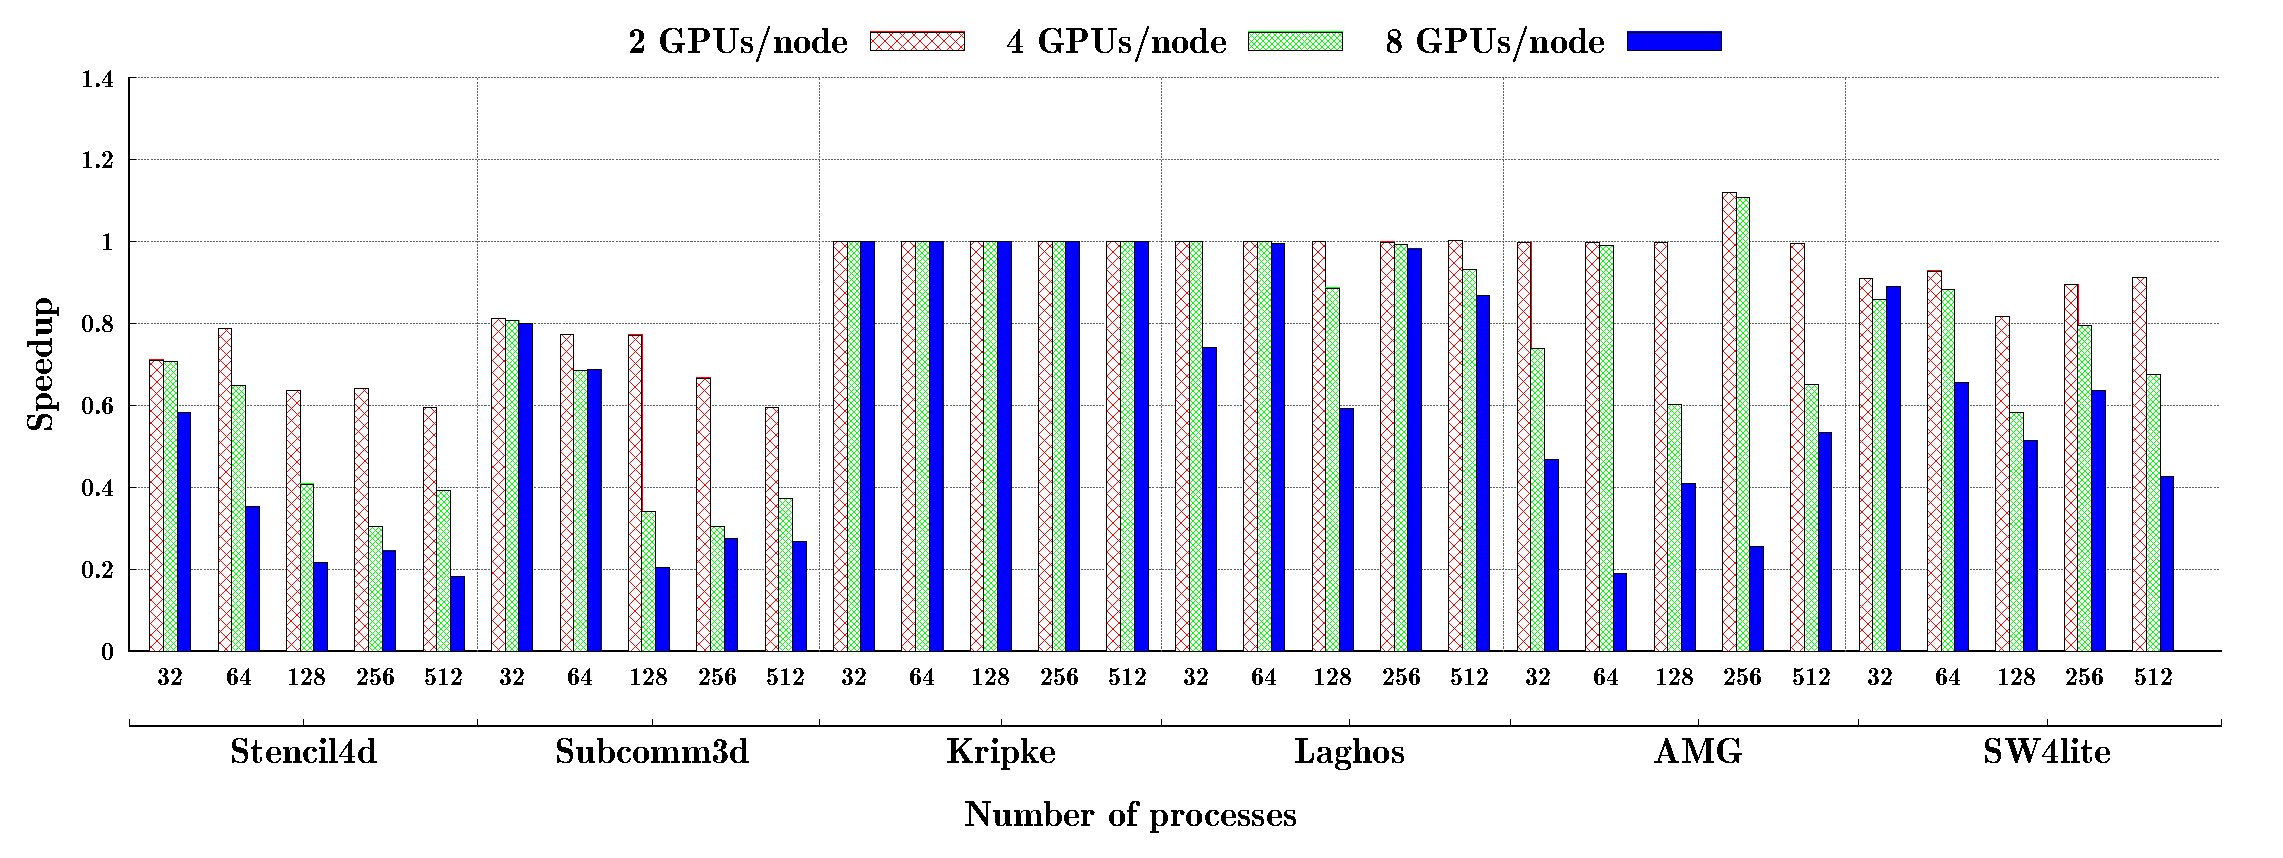
\includegraphics[width=\textwidth]{plots/ftree/map/ftree-mapping-all.eps}
\caption{Speedup on fat-tree for various numbers of GPUs per node settings with
respect to 1 GPU/node configuration.}
\label{fig:ftree_gpu}
\end{figure*}
\FloatBarrier

\FloatBarrier
\begin{figure*}[!htbp]
\centering
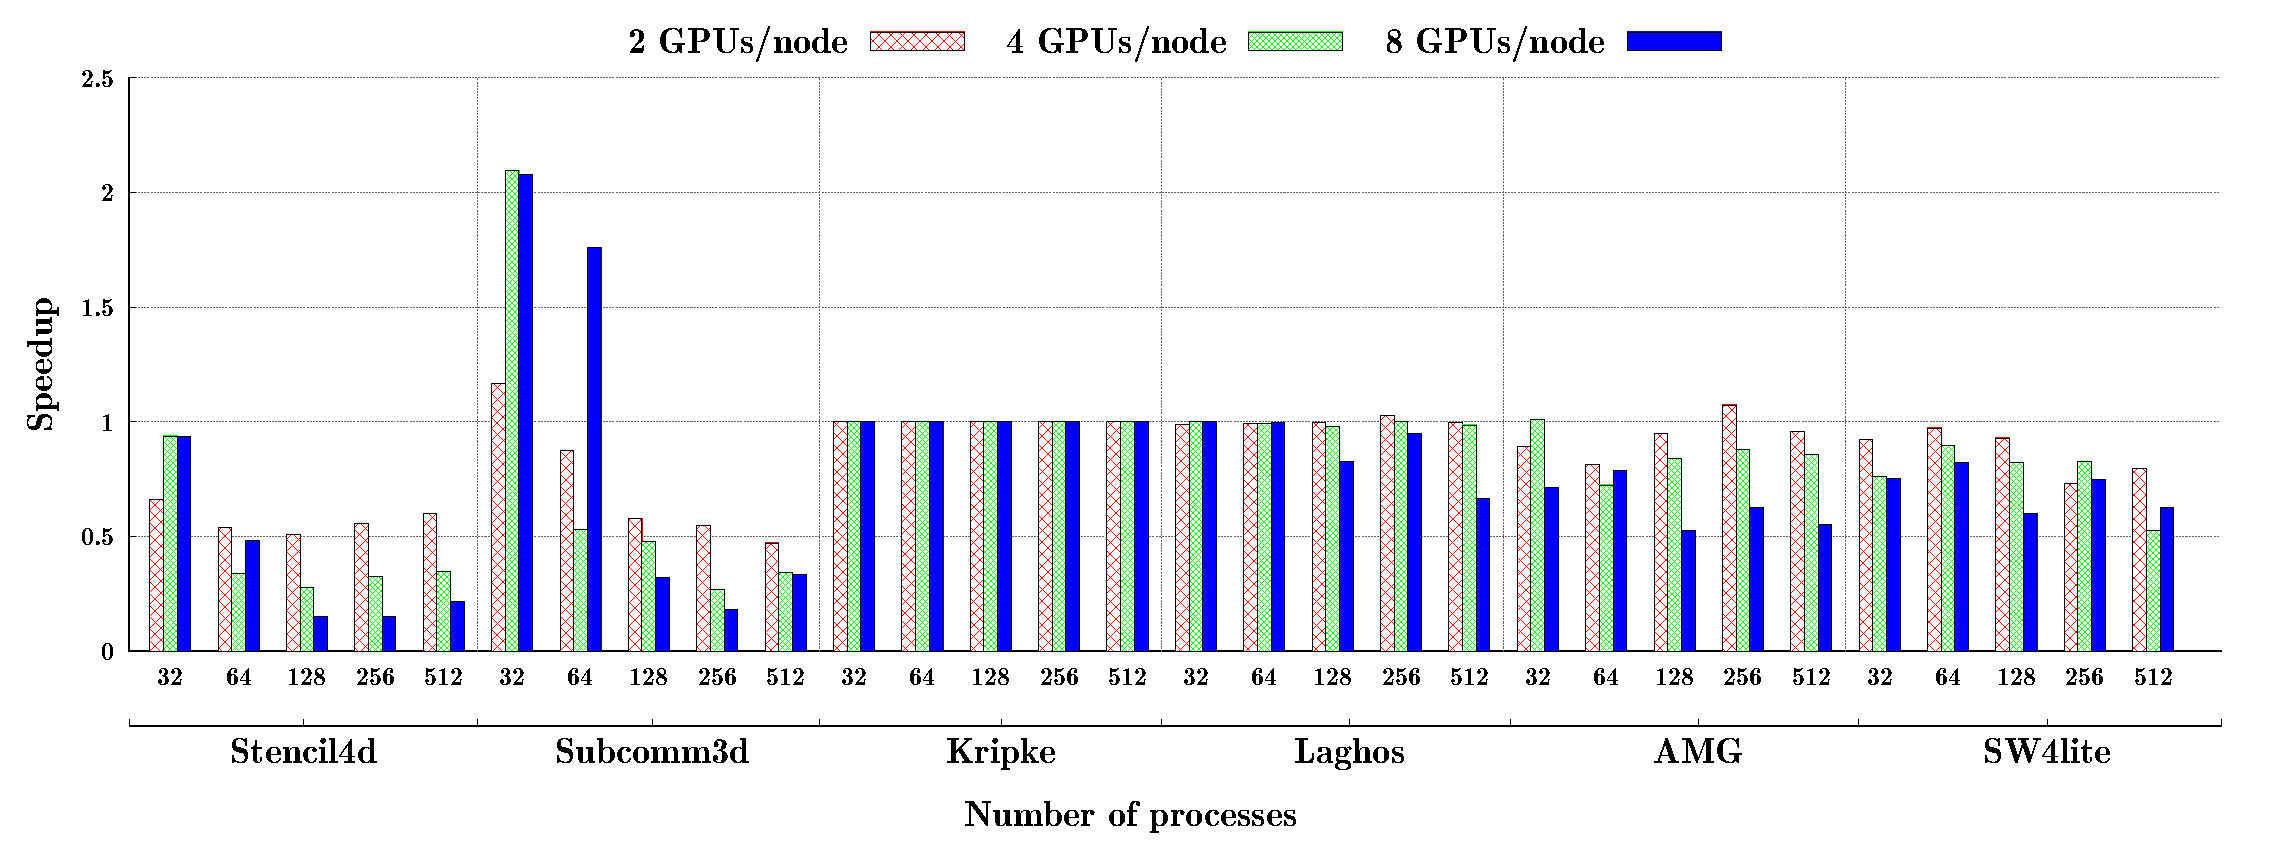
\includegraphics[width=\textwidth]{plots/dfly/map/dfly-mapping-all.eps}
\caption{Speedup on 1D dragonfly for various numbers of GPUs per node settings with
respect to 1 GPU/node configuration.}
\label{fig:dfly_gpu}
\end{figure*}
\FloatBarrier


\subsection{Impact of Network Bandwidth}

In the previous section, as the number of GPUs per node increases, 
the default 1x network bandwidth becomes a performance bottleneck for many
cases is seen.  Thus, the impact of varying network bandwidth along with number of
GPUs/nodes on application performance is studied next. 

\begin{figure}[!htbp]
\centering
    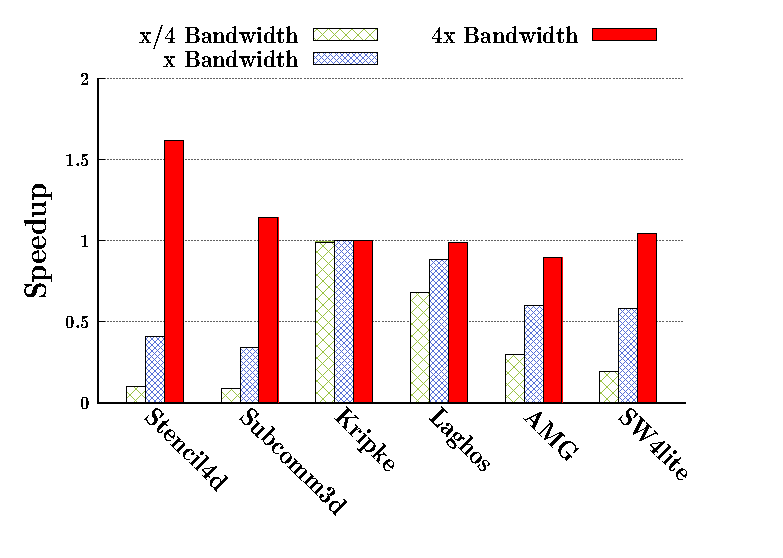
\includegraphics[width=0.8\columnwidth]{figure/plots/bw/ftree-bw-mapping-all.eps}
  \caption{Speedup for the 4 GPUs/node configuration over 1 GPU/node in fat-tree, 1x network
  bandwidth configuration. Data is shown only for job sizes of 128 GPUs.}
  \label{fig:bw_ftree}
\end{figure}

\begin{figure}[!htbp]
\centering
    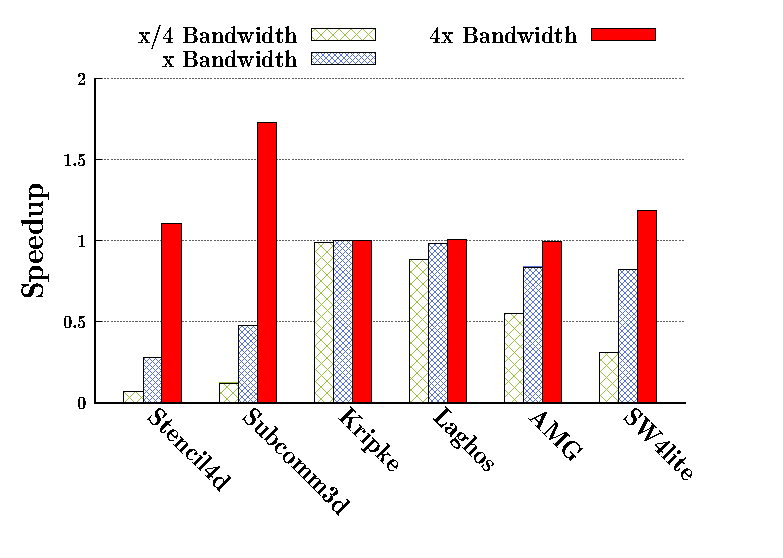
\includegraphics[width=0.8\columnwidth]{figure/plots/bw/dfly-bw-mapping-all.eps}
  \caption{Speedup for the 4 GPUs/node configuration over 1 GPU/node in 1D dragonfly, 1x network
  bandwidth configuration. Data is shown only for job sizes of 128 GPUs.}
  \label{fig:bw_dfly}
\end{figure}

In the simulation experiments, it is observed that the impact of network bandwidth on jobs of different sizes
shares similar trends. Hence, only the data for a job size of 128 processes is presented.
Figure~\ref{fig:bw_ftree} shows the performance for the 4 GPUs per node
configuration with varying network bandwidth relative to 1 GPU per node, 1x
network bandwidth configuration on fat-tree network. We find that the network
bandwidth has a significant impact on most applications.  The gains are  highest
for communication-heavy applications such as Stencil4d and Subcomm3d.
Conversely, the impact of reducing the network bandwidth is also highest for
those.  A similar trend is observed for the 1D dragonfly topology as
shown in Figure~\ref{fig:bw_dfly}.

Table~\ref{tab:bw_ftree} presents the minimum bandwidth required for each
application and a given job size to achieve 90\% of the performance of the
default setting for the fat-tree topology.  As expected, different types of
applications have different bandwidth requirements. In general,
communication-intensive applications require larger bandwidth to sustain the
increased number of GPUs per node while computation-intensive applications have
less bandwidth requirement. For example, for the 8 GPUs per node case with 512 processes
job size, Stencil4d needs 8x network bandwidth
to achieve 90\% of the performance from the default setting; AMG and SW4lite need more than 
4x bandwidth while
Kripke only needs x/8 bandwidth. 

\begin{table}[!htbp]
  \centering
  \caption{Minimum bandwidth required to achieve 90\% of the performance of the
  default 1 GPU/node configuration for fat-tree}
    \label{tab:bw_ftree}
    \vspace{-1em}
    \resizebox{\columnwidth}{!}{%
    \begin{tabular}{lcccc} \toprule
\multirow{2}{*}{Applications}
 & \multicolumn{2}{c}{32 processes}  & \multicolumn{2}{c}{512 processes} \\
\cline{2-5}
& 4 GPUs/node & 8 GPUs/node & 4 GPUs/node & 8 GPUs/node  \\ \midrule
Stencil4d & 1x & 1x & 4x & 8x\\
Subcomm3d & x/2 & x/2 & 4x & 4x\\
Kripke & x/16 & x/16 & x/8 & x/8\\
Laghos & x/2 & 2x & x & 2x\\
AMG & 4x & 8x & 4x & 8x\\
SW4lite & 2x & 2x & 2x & 4x\\ \bottomrule
\end{tabular}
}
\end{table}

Further, application requirements are also affected by the job size and the
placement with other jobs.  For example, 32-process Laghos ran slower in some
workloads when mapped in the 8 GPUs per node configuration, which is why here
double bandwidth is needed to get more than 90\% speedup. It is also seen that sometimes
communication-intensive applications such as Stencil4d and Subcomm3d require
less bandwidth in 8 GPUs per node configuration than 4 GPUs per node
configuration to reach 90\% of the performance for 32 processes and 64 processes.  This
is mainly due to the fact that, with a larger number of GPUs per node, a significant

fraction of the communication happens within the same node.  This indicates that
future GPU-based platforms must consider their workloads to decide important
networking hardware parameters.  The results for 1D
dragonfly, show a similar trend as that in fat-tree. 


\vspace{1em}
\noindent
{\it \textbf{Overall Observation}:
Bandwidth requirement to sustain high performance depends on GPU density
and job sizes.}

\noindent
Our results show that
  each type of application has a sweet-spot for them to perform effectively. 
  Hence, the design of a future GPU cluster should take its applications into
  consideration in order to achieve the maximum performance-cost ratio. 
  %Larger bandwidth allocation compensates slowdown when application is run with more GPUs per node.




\subsection{Impact of Message Scheduling in the NIC}

The impact of message scheduling on system performance has not received
sufficient attention in the community. To my knowledge, this is the first time
that the impact of message scheduling on system and application performance
is being studied systematically.
%The results for application with different numbers of processes have a
%similar trend.
Similar to the impact of the number of GPUs per node and network link bandwidth, the impact
of message scheduling is similar for both fat-tree and 1D dragonfly. Thus,
results for the 1D dragonfly are only discussed in detail. 

%{\bf Sap: check all numbers in this section}
\begin{figure}[!htbp]
  \centering
  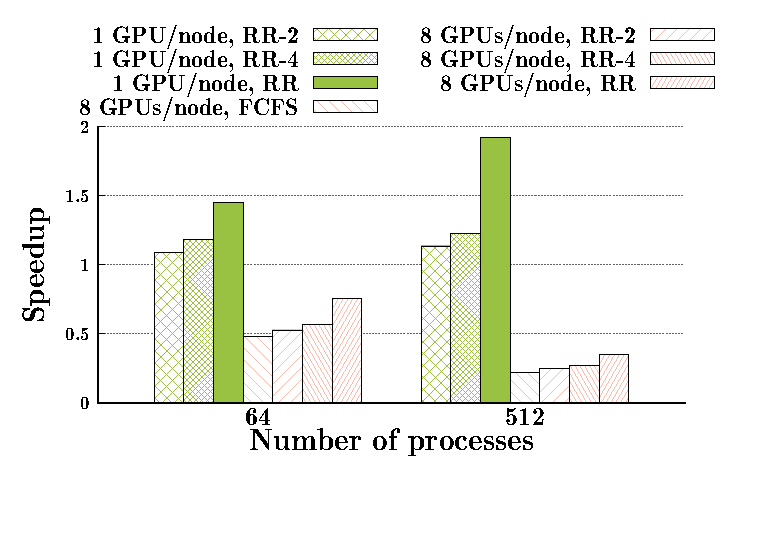
\includegraphics[width=0.8\columnwidth]{figure/plots/sched/dfly-sched-mapping-stencil.eps}
  \vspace{-0.5in}
  \caption{Results for Stencil4d (64 processes and 512 processes on 1D dragonfly)}
  \label{fig:stencil_scheduling_dfly}
\end{figure}


Figure ~\ref{fig:stencil_scheduling_dfly} shows the speedup for 64 and 512
processes (GPUs) of Stencil4d relative to the default case with 1 GPU per node and
FCFS scheduling (network bandwidth is fixed at 1x for all configurations).  For
the 1 GPU per node cases, the scheduling significantly affects the performance:
the larger the number of messages the scheduler considers for packetization
concurrently, the higher the performance. The RR scheduler reaches a speed-up of
1.45 for the 64-process job and 1.93 for the 512-process job in comparison to
the default FCFS scheduler. A similar trend is observed for the 8 GPUs per node
cases: the RR scheduler improves the speed up from 0.48 with the FCFS scheduler to 0.76
for the 64-process job, and from 0.22 to 0.35 for the 512-process job. 

\begin{figure}[!htbp]
\centering
  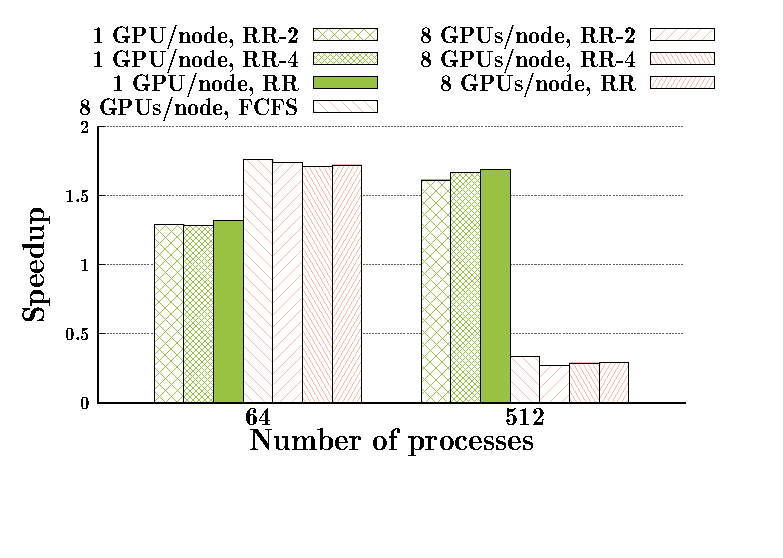
\includegraphics[width=0.8\columnwidth]{figure/plots/sched/dfly-sched-mapping-subcom.eps}
  \vspace{-0.5in}
  \caption{Results for Subcomm3d (64 processes and 512 processes on 1D dragonfly)}
  \label{fig:subcomm3d_scheduling_dfly}
\end{figure}


Figure ~\ref{fig:subcomm3d_scheduling_dfly} shows the speedup for 64 and 512
processes of Subcomm3d.  For 1 GPU per node, RR scheduler performs better
than FCFS. However, RR is only slightly better than RR-2 and RR-4 and achieves a
1.3 speed-up for the 64-process job and 1.7 speed-up for the 512-process job
over FCFS.  For 8 GPUs per node cases, all schedulers have similar performance
with FCFS being slightly better than other scheduling schemes. Although both
Stencil4d and Subcomm3d are communication-intensive, the impact of message
scheduling is different. This is because the communication characteristics in
these two applications are different. 

\begin{figure}[!htbp]
  \centering
  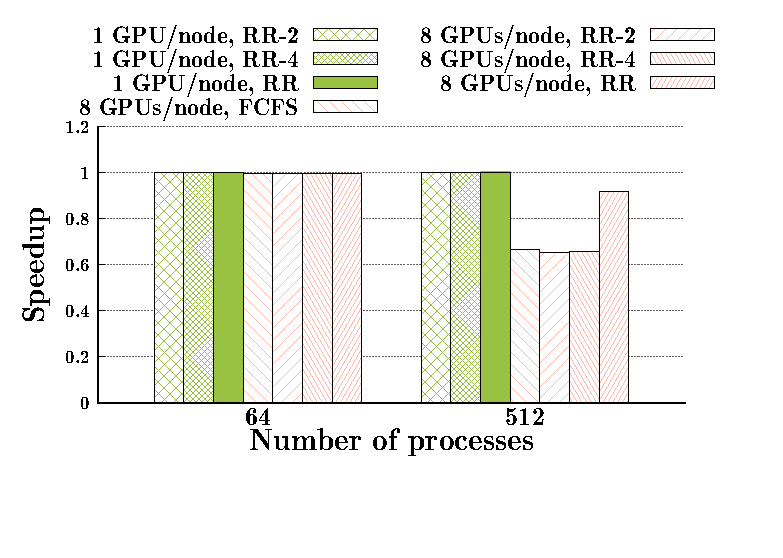
\includegraphics[width=0.8\columnwidth]{figure/plots/sched/dfly-sched-mapping-laghos.eps}
  \vspace{-0.5in}
    \caption{Results for Laghos (64 processes and 512 processes on 1D dragonfly)}
  \label{fig:laghos_scheduling_dfly}
\end{figure}


Message scheduling has no impact on Kripke as Kripke is not sensitive to
communication as seen earlier. Figure~\ref{fig:laghos_scheduling_dfly} shows
the speedup for 64-process and 512-process simulations of Laghos. For 1 GPU per node cases, all
schedulers have the same performance. For 8 GPUs per node cases, all schedulers
have the same performance for the 64-process job, but RR has a significantly
better performance than others for the 512-process job. As shown in
Figure~\ref{fig:dfly_gpu}, for 512 processes (and 256 processes and 128
processes), Laghos is affected by communication only in the 8 GPUs per node
setting.

%\begin{figure}[h]
%  \centering
%  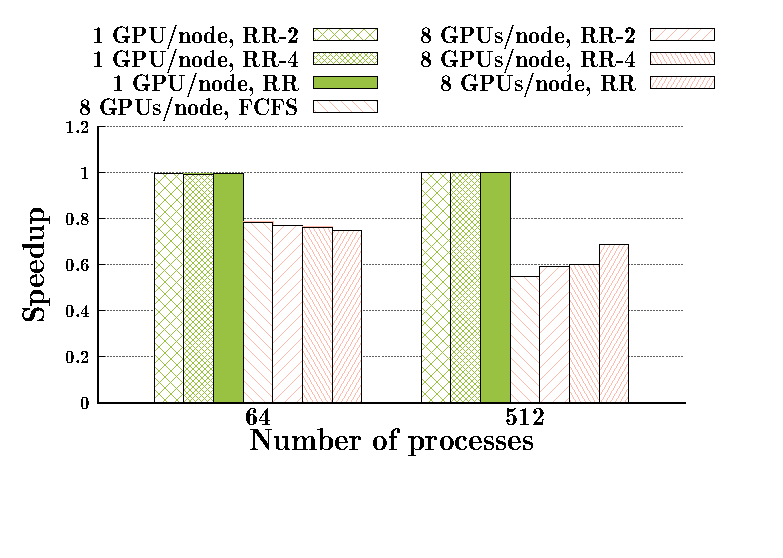
\includegraphics[width=\columnwidth]{figure/plots/sched/dfly-sched-mapping-amg.eps}
%  \vspace{-0.5in}
%    \caption{Results for AMG (64 processes and 512 processes on 1D dragonfly)}
%  \label{fig:amg_scheduling_dfly}
%\end{figure}

\begin{figure}[!htbp]
  \centering
  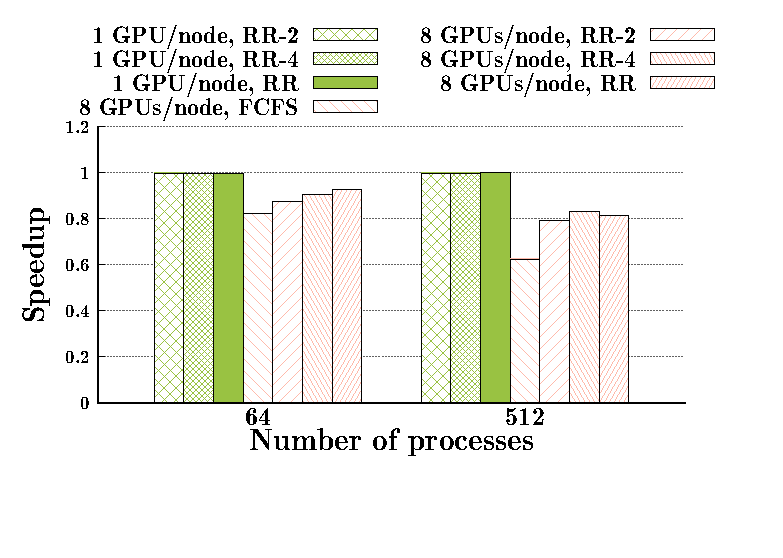
\includegraphics[width=0.8\columnwidth]{figure/plots/sched/dfly-sched-mapping-sw4lite.eps}
  \vspace{-0.5in}
  \caption{Results for SW4lite (64 processes and 512 processes on 1D dragonfly)}
  \label{fig:sw4lite_scheduling_dfly}
\end{figure}


Figures~\ref{fig:sw4lite_scheduling_dfly} show the
results for SW4lite. Message scheduling has no impact on the 1 GPU per node cases, but
affects the performance significantly for 8 GPUs per node cases for both applications and the two
job sizes. The impact, however, depends on both the application and job sizes.
Similar results are seen for AMG application.
%This is due
%to the changing of the inter-node communication characteristics. Simillar results are seen for AMG.

\vspace{1em}
\noindent
{\it \textbf{Overall Observation}:
For most applications, some degree of round robin in NIC scheduling is effective. However
    the exact degree is application dependent -- no single scheduling scheme can achieve the best
  performance across applications.}

Message scheduling can impact performance only when there are many concurrent
communicating pairs. For the 1 GPU per node cases, it thus only affects the
communication heavy applications such as Stencil4d, and has virtually no impact
on the other applications in the study. As the number of GPUs per node
increases, so does the  number of communication sources and the number of
concurrent communications. Thus, with 8 GPUs per node, message scheduling makes
a difference in all applications, except Kripke.  The magnitude of the impact,
however, depends on the application as well as the job size: Round-robin (RR) is
the most effective scheduling in many cases.  However, each of the scheduling
schemes achieves the best performance in some cases.
For example, FCFS is the best for AMG with 64 processes and 8 GPUs per node;
RR-4 is slightly better than other scheduling policies for SW4lite with 512
processes and 8 GPUs per node.  The effectiveness of message
scheduling depends on both application and the network parameters, and needs to
be further studied by examining more applications as well as system
configurations. 



